\chapter{Manifold Learning by Deep Learning}
\label{sec:manifold}

\section{Introduction}

% Start with section on manifold learning of AD and MS
% populations. Including a summary of those methods and the whole literature
% review of what has been done. This includes manifold learning, population
% studies, disease classification and the likes without deep learning.

\begin{comment}

What is manifold learning?

Why are we doing it?


\end{comment}

% In this chapter, we will use manifold learning to detect patterns of variability
% in groups of images. Variability is captured in terms of the coordinates in
% manifold space, which can be used as imaging biomarkers for assessing the
% disease state or for classification into different subtypes. In this chapter, we
% propose using a deep learning model called a deep belief network for learning
% the manifold of medical images. The potential of deep learning for manifold
% learning was evaluated on images of AD patients and MS patients.

Changes in brain morphology such as global and regional atrophy and the
formation of white matter lesions are two hallmarks of \gls{ms} pathology. In
order to quantify the pathological manifestation of MS, a number of imaging
biomarkers derived from \gls{mri} scans of the brain, such as lesion volume and
whole brain volume, have been proposed, which have established their importance
for the study of MS. However, MS is a complex disease whose pathological
variability extends well beyond what can be captured by global and local
volumetric measures. It would be highly desirable to have a method that can
automatically discover potentially important patterns of variability in brain
morphology and lesion distribution, which would advance our understanding of the
complex pathology of MS. In addition, the joint modeling of brain morphology and
lesion distribution would further our knowledge of how these two key
pathological features interact. However, this type of modeling is very
challenging due to the high dimensionality of the data.

In recent years, there has been an increased interest in biomarker discovery
using manifold learning to form high-level, low-dimensional representations of
medical images \citep{wolz2010b,aljabar2011,wolz2012}. In order to discover
common patterns of variability in a group of images, each image of the data set
is regarded as a point in a high-dimensional image space (called the ambient
space), with $n_x \times n_y \times n_z$ coordinates, where $n_x, n_y, n_z$ are
the dimensions of each image. On the other hand, each image could also be
identified by a smaller set of parameters that describe shape variations and
patterns that are common for a particular group of images. These parameters span
a new space called the manifold space. The task of manifold learning is to
discover the low-dimensional space and its parameters, which can then be used to
model the anatomical variability within a population, or serve as biomarkers to
track disease state and progression.

In the remainder of this section, we will briefly revise common manifold
learning techniques and applications for medical image analysis. A main part of
the chapter will be an explanation of the deep learning manifold learning
framework using a deep belief network. We have evaluated the proposed manifold
learning method on two tasks: a) to learn the variability of \gls{mr} images of
the brain of \gls{ad} patients, and b) to discover patterns of morphological
variability and lesion distribution in MS.

\section[Manifold learning for medical image analysis]{Manifold Learning for
Medical Image Analysis}

Most popular manifold learning methods for medical image analysis can be roughly
classified into local and global methods \citep{cayton2005}. Local algorithms
such as \gls{lle} \citep{saul2003} and \gls{lem} \citep{belkin2002} try to find a low
dimensional representation of the data such that local distances between points
in ambient space are best preserved when mapped to manifold space. In contrast,
global methods such as \gls{isomap} \citep{tenenbaum2000} try to find an
embedding of the manifold space that best preserves geodesic distances of points
that lie far apart in ambient space. Both types of methods require building a
proximity graph that is used to capture neighborhood information (local methods)
or to estimate geodesic distances by calculating the shortest path distances
between all points on the affinity graph (global methods). Both types of methods
assume that the manifold is locally linear, which means that distances between
neighboring points in manifold space can be approximated by their distances in
ambient space. Once the proximity graph has been created, a unique solution to
the inherent optimization problem of each algorithm can be found analytically by
solving an eigenvalue problem.

\begin{comment}

Applications:
- regularize segmentation of the heart ventricles
- regularize segmentation of the brain ventricles
- constrain registration
- clinical predictions
- biomarker discovery
- atlas propagation for the segmentation of the hippocampus
- discriminate between normal and abnormal motion patterns of the heart
- feature extraction
- similarity measure for images -> prediction of AD
- classification of Alzheimer's disease
- extract features representing inter-subject variability

\end{comment}

Manifold learning methods have been successfully applied to various image
analysis problems such as the segmentation of the hippocampus \citep{wolz2010},
to regularize the segmentation of heart \citep{zhang2006} and brain
ventricles~\citep{etyngier2007}, and to constrain the deformable registration of
brain images to have biologically plausible parameters \citep{hamm2010}, while
most methods focus on clinical prediction
\citep{gerber2010,wolz2012,duchateau2012,aljabar2011,wachinger2015,bhatia2012,
guerrero2014}. Gerber et al. used Isomap to predict clinical parameters of AD
patients \citep{gerber2009,gerber2010}, and Wolz et al. used LEM to perform
biomarker discovery \citep{wolz2011,wolz2012}, also of AD patients.
\citet{duchateau2011,duchateau2012} discriminate between normal and abnormal
motion patterns of the heart based on the definition of pathology as a deviation
from normality. After learning the manifold representing normal motion
patterns, abnormal motion patterns can be detected based on the
distance of a new data sample from the manifold surface.
% \citet{aljabar2010,aljabar2011} proposed a method for the joint modeling of
% multiple image features of neonatal brains. First, separate manifolds based on
% features from geometric surface models, non-rigid deformations, and image
% intensities are learned, then a second dimensionality reduction step is used
% to combine the individual manifold parameters.
\citet{wachinger2015} proposed a new shape descriptor of the brain called
BrainPrint, which is build by solving the eigenvalue problem of the 2D and 3D
Laplace-Beltrami operator on meshes of segmented cortical and subcortical
structures. The descriptor defines a similarity measure on brain images, which
can be used to perform subject identification \citep{wachinger2014a}, and to
predict Alzheimer's disease \citep{wachinger2014b}.
\citet{bhatia2012} model regional variations of the brain by building a manifold
on hierarchical image patches and applied it to finding discriminative regions
of 3D brain \gls{mr} images for classifying Alzheimer's disease.
\citet{guerrero2014} have used manifold learning on \glspl{roi} to
extract features that represent inter-subject variability of AD patients.
In a first step, sparse regression is used to automatically detect the
\gls{roi} using \gls{mmse} scores as the independent
variable. Then, LEM with cross-correlation as the distance measure is used to
learn the manifold of the ROIs, from which the features are extracted.

A main challenge of most manifold learning methods (e.g., Isomap, LEM, LLE) is
the construction of the proximity graph. Building the proximity graph requires
choosing an appropriate neighborhood criterion, which can be challenging due to
the sensitivity to noise of commonly used criteria (e.g., $k$-nearest neighbors,
$\epsilon$-ball), and, consequently, may result in an unstable topology of the
learned manifold \citep{balasubramanian2002}. Other challenges include avoiding
erroneously disconnected regions and shortcuts, finding a trade-off between
sampling density and curvature of local patches of the manifold, and finding a
suitable distance metric. A number of solutions have been proposed, but there is
no general solution. To increase the robustness to noise and varying parameter
settings, \citet{carreira2005} proposed building the graph from a graph ensemble
that combines multiple spanning trees, each fit to a perturbed version of the
data set. A trade-off between sampling density and curvature of local patches of
the manifold can be found automatically by adapting the selection of the
neighborhood sizes through neighborhood contraction and expansion
\citep{zhang2012}. \citet{gerber2010} have shown that the choice of a suitable
distance measure is crucial for manifold learning using Isomap and that the
warping distance between brain images improves the learning performance over
previously used Euclidean distances in the image space.

\section[Manifold learning using deep belief networks]{Manifold Learning using
Deep Belief Networks}

Deep generative models such as \glspl{dbn} are a promising alternative to
previously used brain manifold learning methods due to their ability to discover
patterns of similarity in groups of images. In contrast to most commonly used
manifold learning algorithms (e.g., LLE, LEM, Isomap), DBNs do not assume the
manifold space to be locally linear and do not require a previously defined
similarity measure or the construction of a proximity graph, which makes them
more generally applicable to a wide range of manifold learning tasks. This is
particularly important for the application to brain manifold learning, because
the high-dimensionality of brain MRIs make defining a neighborhood criterion
challenging.

% DBNs have been used for many
% different tasks where the choice of an appropriate architecture is crucial for
% the success. In this section, we will explain the choices we made in designing
% the overall manifold learning framework. Particular parameter choices are
% explained along with two applications.

\subsection[General architecture]{General Architecture}
\label{sec:general_arch}

The general architecture of the DBN used for manifold learning of brain MRIs is
illustrated in \ref{fig:manidbn}. The first \gls{rbm} receives the intensity
values of a group of images in ambient space as input and reduces the
dimensionality of each image by discovering patterns of similarity that are
common within groups of images. Subsequent RBMs receive the hidden unit
activations of the previous RBM as input, thus learning successively more
complex and abstract patterns from a training set, where the hidden units of the
last layer represent the coordinates of an image in manifold space. The number
of trainable weights increases significantly with the resolution of the training
images. In order to scale the model to high-resolution images, the first several
layers of our DBN are \glspl{scrbm}, a type of RBM that uses weight sharing and
local connectivity between units of adjacent layers to reduce the number of
trainable weights. Due to the much smaller number of trainable parameters
compared to dense RBMs, sconvRBMs are best suited for learning low- to mid-level
features from very high-dimensional data such as brain MRIs. Compared to other
more commonly used convolution-based RBMs \citep{lee2009}, an advantage of
sconvRBMs is that inference is invertible, which allows the reconstruction of
the visible units from the hidden unit activations. In our application, this
allows for the mapping of parameters from the manifold space back to the ambient
space. Due to the local connectivity of the weights, sconvRBMs can only learn
local patterns in the data. In order to learn patterns that describe images as a
whole, sconvRBM layers are followed by dense RBMs, which integrate the extracted
feature from all image locations in order to model global patterns.

\begin{figure}
\centering
\begin{tikzpicture}[scale=0.85]
\tikzstyle{every node}=[font=\sffamily\small, inner sep=3pt, align=center]
\tikzstyle{every pin}=[align=center,fill=white,overlay]
\tikzstyle{dbnlabel}=[font=\sffamily]
         
% Deformation field
        
%\node[dbnlabel, rotate=90] at (-1.5,2.25) {Morphology DBN};
        
\begin{scope}[xshift=-10pt,yslant=0.63,xscale=0.4]

\node[transform shape,pin={[pin
distance=8]125:Input image}] (field) at (2,2)
{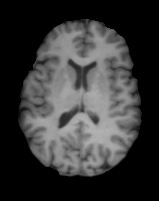
\includegraphics[width=3.45cm]{figures/MICCAI2015_CHB07-T1w-s88}};

% \node[pin={[pin distance=0.6,overlay]93:Displacement\\
% field $u$}] at ($(field.north west)!0.1!(field.north east)$) {};

\end{scope}
         
% 3-channel input

\foreach \x in {20} {
\begin{scope}[xshift=\x pt]
%\ifnum\x=0
%\path
%\else
\draw[fill=white, fill opacity=0.75]
%\fi
  (0,0) coordinate(A\x) -- ++(90:4) coordinate (B\x) -- ++(30:2) coordinate
  (C\x) -- ++(-90:4) -- cycle;
  

% \begin{scope}[xshift=-50pt,yslant=0.63,xscale=0.4]  
% \node[transform shape,inner sep=0pt] at (2,2)
%   {\includegraphics[width=4cm]{deformation2.png}};
% \end{scope}
  
\draw (0,3)
   ++(30:0.25) \ifnum\x=20 coordinate (a1) \else -- +(0:10pt) +(0:0) \fi
-- ++(90:0.5)  \ifnum\x=20 coordinate (b1) \else -- +(0:10pt) +(0:0) \fi
-- ++(30:0.25) \ifnum\x=20 coordinate (c1) \else -- +(0:10pt) +(0:0) \fi
-- ++(-90:0.5) \ifnum\x=20 coordinate (d1) \else -- +(0:10pt) +(0:0) \fi
-- ++(210:0.25);
\end{scope}
}

%\node[below=4pt,xshift=-3pt] at (A0)  {$u_x$};
%\node[below=4pt] at (A10) {$u_y$};
%\node[below=4pt,xshift=3pt] at (A20) {$u_z$};

%\node[pin={[pin distance=5pt]260:$u_x$}] at (A0)  {};
%\node[pin={[pin distance=5pt]270:$u_y$}] at (A10)  {};
%\node[pin={[pin distance=5pt]290:$u_z$}] at (A20)  {};

\draw[decorate,decoration={brace,raise=4pt,mirror}]
(A20) --node[below=8pt] {Visible units} (A20-|C20);

% Transition

\draw ($(a1)!0.5!(c1)$) ++(55pt,-5pt) coordinate (e1);
\draw (a1) -- (e1);
\draw (b1) -- (e1);
\draw (c1) --node[pin={[pin distance=1cm]40:Strided\\ convolution}] {} (e1);
\draw (d1) -- (e1);

% First layer hidden units

\foreach \x in {80,85,90,95,100,105} {
\begin{scope}[xshift=\x pt,yshift=1.5cm,scale=0.5]
\draw[fill=white, fill opacity=0.75]
  (0,0) coordinate(A\x) -- ++(90:4) coordinate (B\x) -- ++(30:2) coordinate
  (C\x) -- ++(-90:4) coordinate(D\x) -- cycle;
   
\draw (0,2.5)
   ++(30:0.25) \ifnum\x=105 coordinate (a2) \else -- +(0:10pt) +(0:0) \fi
-- ++(90:1)    \ifnum\x=105 coordinate (b2) \else -- +(0:10pt) +(0:0) \fi
-- ++(30:0.5)  \ifnum\x=105 coordinate (c2) \else -- +(0:10pt) +(0:0) \fi
-- ++(-90:1)   \ifnum\x=105 coordinate (d2) \else -- +(0:10pt) +(0:0) \fi
-- ++(210:0.5);
\end{scope}
}

\draw[decorate,decoration={brace,raise=20pt}] (B20|-C20) --node[above=25pt]
{Strided convolutional RBM} (C105|-C20);

%\draw[decorate,decoration={brace,raise=4pt,mirror}]
%(A80) --node[below=8pt] {$N = 32$} (A80-|D105);
%(A80) --node[below=8pt] {Hidden units} (A80-|D105);

\draw ($(a2)!0.5!(c2)$) ++(0:38pt) coordinate (e2);
\draw (a2) -- (e2);
\draw (b2) -- (e2);
\draw (c2) -- (e2);
\draw (d2) -- (e2);

% Second layer hidden units

\foreach \x in {145, 150, ..., 175, 180} {
\begin{scope}[xshift=\x pt,yshift=2.25cm,scale=0.25]
\draw[fill=white, fill opacity=0.75]
  (0,0) coordinate(A\x) -- ++(90:4) coordinate (B\x) -- ++(30:2) coordinate
  (C\x) -- ++(-90:4) coordinate(D\x) -- cycle;
\draw (0,1.75)
   ++(30:0.25) \ifnum\x=180 coordinate (a3) \else -- +(0:20pt) +(0:0) \fi
-- ++(90:2)    \ifnum\x=180 coordinate (b3) \else -- +(0:20pt) +(0:0) \fi
-- ++(30:1)    \ifnum\x=180 coordinate (c3) \else -- +(0:20pt) +(0:0) \fi
-- ++(-90:2)   \ifnum\x=180 coordinate (d3) \else -- +(0:20pt) +(0:0) \fi
-- ++(210:1);
\end{scope}
}

%\draw[decorate,decoration={brace,raise=4pt,mirror}]
%(A145) --node[below=8pt] {$N = 64$} (A145-|D180);

\draw ($(a3)!0.5!(c3)$) ++(0:18pt) coordinate (e3);
\draw (a3) -- (e3);
\draw (b3) -- (e3);
\draw (c3) -- (e3);
\draw (d3) -- (e3);

% Third layer hidden units

\foreach \x in {200, 205, ..., 240} {
\begin{scope}[xshift=\x pt,yshift=2.625cm,scale=0.125]
\draw[fill=white, fill opacity=0.75]
  (0,0) coordinate(A\x) -- ++(90:4) coordinate (B\x) -- ++(30:2) coordinate
  (C\x) -- ++(-90:4) coordinate(D\x) -- cycle;
\end{scope}
}

% Forth layer visible units (dense)

\begin{scope}[xshift=280pt, yshift=2.75cm]
\foreach \x/\y in {0/-2, 1/-1.5, 2/-1, 3/-0.5, 4/0, 5/0.5, 6/1, 7/1.5, 8/2} {
  \node[circle, draw] (v\x) at (0,\y) {};
}
\end{scope}

\draw[shorten >=10pt,shorten <=10pt,dashed] (A240)--(v0.south west);
\draw[shorten >=10pt,shorten <=10pt,dashed] (A240|-C240)--
node[label=120:Vectorize] {} (v8.north west);

\node[fit=(v0), pin={[pin distance=10pt]240:Vectorized\\hidden units}] {};

\draw[decorate,decoration={brace,raise=4pt,mirror}]
(A80) --node[below=8pt,fill=white] {%
Hidden units of \\
sconvRBMs}
(A80-|D240);

%\node[rotate=90,fill=white,align=center] at(270pt,2.75cm) {Serialize\\ hidden
%units};

% Forth layer hidden units (dense)

\begin{scope}[xshift=320pt, yshift=2.75cm]
\foreach \x/\y in {0/-1, 1/-0.5, 2/0, 3/0.5, 4/1} {
  \node[circle, draw] (h\x) at (0,\y) {};
}
\end{scope}

\foreach \x in {0, ..., 8} {
  \foreach \y in {0, ..., 4} {
    \draw[very thin] (v\x)--(h\y);
  }
}

\draw[decorate,decoration={brace,raise=20pt}] (v8.west|-C20)
--node[above=25pt] {Dense RBM} (h0.east|-C20);

% Fifth layer hidden units (distribution parameters)

\begin{scope}[xshift=360pt, yshift=2.75cm]
\foreach \x/\y in {1/0.25, 2/-0.25} {
  \node[circle, draw, label=0:$M_\x$] (D\x) at (0,\y) {};
}
\end{scope}

\foreach \x in {0, ..., 4} {
  \foreach \y in {1,2} {
    \draw[very thin] (h\x)--(D\y);
  }
}

\draw[decorate,decoration={brace,raise=10pt,mirror}]
(h0.west|-h0.south) --node[below=14pt,fill=white] {%
Hidden units of\\ dense RBMs}
(h0.south-|D1);

% \draw[decorate,decoration={brace,raise=22pt}]
% (D1.north-|D1.east) --node[above,sloped] {Deformation\\ parameters}
% (D2.south-|D2.east);

\end{tikzpicture}

\caption[General architecture of the DBN used to learn the manifold of brain
MRIs]{General architecture of the DBN used to learn the manifold of brain
MRIs. The visible units of the DBN represent the intensity values of images in
ambient space. The hidden units of the last layer represent the image
coordinates in manifold space ($M_1, M_2$). The first several layers of the DBN
are sconvRBMs followed by one or more dense RBM layers.}

\label{fig:manidbn}
\end{figure}

\subsection[Unit types]{Unit Types}

To apply the model to real-valued data like the intensities of some medical
images, the visible units are modeled as Gaussian units. As suggested in Hinton
et al.'s RBM training guide \citep{hinton2010a}, we did not learn the variance
of the Gaussian units and standardized the inputs to having zero mean and unit
variance instead. There are two typical choices for the hidden units of an RBM,
binary hidden units and \glspl{nrelu}. A binary hidden unit can only encode two
states. In order to learn patterns of variability that span a continues spectrum
of changes instead of binary on/off patterns, we use NReLUs as the hidden
units, which have also shown to improve the learning performance
\citep{nair2010} of RBMs.

\subsection[Incorporating a region of interest]{Incorporating a Region of
Interest}

A challenge for training DBNs on brain MRIs is that large black regions
without local structure can lead to random activations of the hidden units and
consequently to the learning of random filters. To overcome this problem, we
propose incorporating a \gls{roi} term into the energy equation of the
\gls{crbm}, which allows constraining the filter learning process to a given
ROI. This can be achieved by the element-wise multiplication of the visible and
hidden units with a binary mask, which sets the visible and hidden units outside
of the ROI to zero, thereby removing their contribution to the energy of the
model. The modified energy of the model is given by
\begin{align} 
\nonumber
E(\vect{v},\vect{h}, \vect{r}_\text{v}, \vect{r}_\text{h}) =
&-\sum_{i=1}^{N_\text{c}} \sum_{j=1}^{N_\text{k}}
(\vect{r}_\text{h} \cdot \vect{h}^{(j)}) \bullet
(\tilde{\vect{w}}^{(ij)} * (\vect{r}_\text{v} \cdot \vect{v}^{(i)}))\\
&- \sum_{i=1}^{N_\text{c}}b_i\sum_{x,y = 1}^{N_\text{v}}%
\!r_{\text{v},xy}v_{xy}^{(i)}
- \sum_{j=1}^{N_\text{k}}c_j\sum_{x,y = 1}^{N_\text{h}}%
\!r_{\text{h},xy}h_{xy}^{(j)},
\end{align}
where $\vect{r}_\text{v}$ and $\vect{r}_\text{h}$ are binary masks defining the
ROI with respect to the visible and hidden units, and $\cdot$ denotes
element-wise multiplication. Because sconvRBMs can be mapped to equivalent
convRBMs, we can use the same modification to restrict the learning of filters
of sconvRBMs.

% TODO: (Optional) add modified equations for inference

% A major constraint for designing a DBN for manifold learning is the amount of
% memory required for storing the hidden units. Although the application of
% strided convolutions as part of the sconvRBM decreases the size of a single
% channel, filtering in the first sconvRBM increases the number of channels due to
% the application of multiple filters. Choosing a stride size of 4 reduces the
% amount of memory required for storing one channel by 32, which allows the use of
% 32 filters without requiring more memory to store the hidden units. For
% subsequent layers, we chose a stride size of 2, which roughly halves the size of
% each dimension of a channel. We choose a smaller stride size in the
% $z$-dimension to roughly compensate of the anisotropic voxel size of the images
% used in our experiments.

% TODO: shorten it a bit and give more intuition behind it, why do we model it
% like this?

\section[Manifold of MRIs of Alzheimer's disease patients]{Manifold of MRIs of
Alzheimer's Disease Patients}

% Motivation and short overview of the method and why use this one and not
% alternatives. What data was used? Applied to RAW MRI images without much
% preprocessing.

In a first experiment, we applied our manifold learning framework using DBNs to
the task of learning the manifold of brain MRIs of AD and healthy subjects. DBNs
have shown to be able to learn the manifold of handwritten digits
\citep{hinton2006b} or small natural images \citep{krizhevsky2010}. However,
those data sets contain a large number of small images, where the number of
images (number of data points) well exceeds the number of pixels per image (the
dimension of a data point). For this experiment, we were interested if DBNs are
able to learn the manifold of images without overfitting, when the dimension of
a data point well exceeds the number of data points, as is commonly the case for
biomedical data sets. A second question was if DBNs can learn meaningful
patterns despite the limited amount of training data.

% This paper is the first to show how training can be accelerated in order
% to train DBNs on full-resolution 3D medical images and that DBNs are able to
% learn a low-dimensional manifold of brain volumes that detects modes of
% variation that correlate to demographic and disease parameters.

\subsection[Data sets and preprocessing]{Data Sets and Preprocessing}

We have evaluated the proposed method on a subset of the \gls{adni} data set
\citep{petersen2010}, containing 300 \gls{t1w} MRIs of \gls{ad} and normal
subjects. The images were provided skull-stripped and bias field corrected. We
resampled all images to a resolution of \num{128x128x128} voxels and a voxel
size of \SI{2.0x2.0x2.0}{\milli\meter}. We then normalized their intensities to
a common range, and rigidly registered them to a group-wise mean image prior to
training and testing. We did not perform non-rigid registration for spatial
normalization in order to evaluate the capabilities of the method without the
added confound of complex registration parameters. The data set was divided into
a training set and a test set such that each set contains 75 AD and 75 normal
subjects.

\subsection{Method}

To learn the manifold of brain MRIs, we used a DBN with three sconvRBM layers
and two dense \gls{rbm} layers as described in \ref{sec:general_arch}. The
parameters of the DBN were chosen to yield a continuous reduction of the
dimensionality of the input images and are summarized in \ref{tab:adni_param}.
For this experiment, we used circular convolutions instead of valid convolutions
for the training of the sconvRBMs, which is a type of convolution that does not
reduce the output size by the filter size. This simplifies the choice of
parameters of the DBN, because the sizes of the hidden layers are independent of
the filter sizes. For the first layer, we chose a stride size of \num{4x4x4},
which results in a strong reduction of the dimensionality in order to reduce the
amount of memory required to train the second layer. Increasing the stride size
decreases the overlap of adjacent sliding windows. To compensate, we also chose
a larger filter size for the first layer than for all subsequent layers. After
the application of three sconvRBMs, the dimension of each image is reduced to
\num{8x8x8} and small enough for RBMs. The training of the DBN took
approximately 43 hours on two GeForce GTX 560 Ti graphics cards.

% Explain the method in more detail. Also what tools where used for the
% experiments and stuff. How was the DBN designed and why.

\begin{table}
\centering
\caption{Parameters of the DBN used to learn the manifold of brain MRIs of AD
and healthy subjects.}
\label{tab:adni_param}
\small
\begin{tabular}{lcccc}
\toprule
Layer type & Kernel size & Stride size & \#Filters/ & Output size \\
           &             &             & \#Hidden units \\
\midrule
Input      & --- & --- & --- & \num{128x128x128x1} \\
\addlinespace
sconvRBM1  & \num{20x20x20x1}\phantom{0} & \num{4x4x4} & 32 & \num{32x32x32x32}
\\
sconvRBM1  & \num{14x14x14x32} & \num{2x2x2} & 32 & \num{16x16x16x32} \\
sconvRBM1  & \num{10x10x10x32} & \num{2x2x2} & 64 & \num{8x8x8x64} \\
\addlinespace
RBM1       & --- & --- & 32 & \num{32} \\
RBM2       & --- & --- & 2  & \num{2} \\
\bottomrule
\end{tabular}
\end{table}

\subsection{Results}

\subsubsection{Geometric Fit of the Manifold}

The geometric fit of the learned manifold model was evaluated in terms of the
generalizability to new images and the specificity to images from the training
set. The generalizability was measured in terms of the average \gls{rmse}
between images $I$ and their reconstructions $R$, normalized by the intensity
range of the input images
\begin{equation}
\text{RMSE} = \frac{\sqrt{\frac{1}{N}\sum_{\vect{p}} (I(\vect{p}) -
R(\vect{p}))^2}}{\max(I)-\min(I)},
\end{equation}
where $\vect{p}$ denotes the coordinates of a particular voxel of an image and
$N$ denotes to total number of voxels. The specificity was measured by
calculating the average RMSE between images randomly generated from the manifold
model using block Gibbs sampling and the most similar images from the training
set. \ref{fig:genspe} shows a comparison of the reconstruction errors between
the training and test sets, and the specificity at different layers of the DBN.
The similarity of the reconstruction errors between the training and test images
indicates that no overfitting is occurring. The average reconstruction error at
the last layer is below \SI{6}{\percent}. Even though the very small
reconstruction error is partially due to head MRIs having a large amount of
homogeneous background, it demonstrates the ability of the learned manifold to
capture most of the visual information with only two manifold parameters. The
opposite slopes of the reconstruction errors and error of generated images
indicates a trade-off between generalizability and specificity in the earlier
phases of training. The low errors at the end of training (layer 5) indicates
that the method is able to be both specific and generalizable.

\begin{figure}[tb]
\centering
%% Created by tikzDevice version 0.6.2-92-0ad2792 on 2013-06-06 10:46:52
% !TEX encoding = UTF-8 Unicode
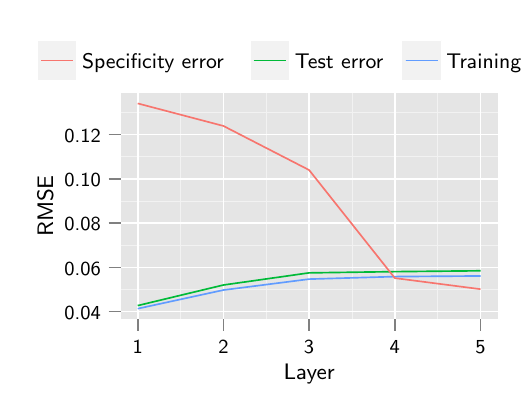
\begin{tikzpicture}[x=1pt,y=1pt]
\tikzstyle{clip}=[]
\definecolor[named]{fillColor}{rgb}{1.00,1.00,1.00}
\path[use as bounding box,fill=fillColor,fill opacity=0.00] (0,0) rectangle (169.83,130.09);
\begin{scope}
\path[clip] ( 33.55, 24.84) rectangle (169.83,106.43);
\definecolor[named]{fillColor}{rgb}{0.90,0.90,0.90}

\path[fill=fillColor] ( 33.55, 24.84) rectangle (169.83,106.43);
\definecolor[named]{drawColor}{rgb}{0.95,0.95,0.95}

\path[draw=drawColor,line width= 0.3pt,line join=round] ( 33.55, 35.47) --
	(169.83, 35.47);

\path[draw=drawColor,line width= 0.3pt,line join=round] ( 33.55, 51.46) --
	(169.83, 51.46);

\path[draw=drawColor,line width= 0.3pt,line join=round] ( 33.55, 67.46) --
	(169.83, 67.46);

\path[draw=drawColor,line width= 0.3pt,line join=round] ( 33.55, 83.45) --
	(169.83, 83.45);

\path[draw=drawColor,line width= 0.3pt,line join=round] ( 33.55, 99.44) --
	(169.83, 99.44);

\path[draw=drawColor,line width= 0.3pt,line join=round] ( 55.23, 24.84) --
	( 55.23,106.43);

\path[draw=drawColor,line width= 0.3pt,line join=round] ( 86.21, 24.84) --
	( 86.21,106.43);

\path[draw=drawColor,line width= 0.3pt,line join=round] (117.18, 24.84) --
	(117.18,106.43);

\path[draw=drawColor,line width= 0.3pt,line join=round] (148.15, 24.84) --
	(148.15,106.43);
\definecolor[named]{drawColor}{rgb}{1.00,1.00,1.00}

\path[draw=drawColor,line width= 0.6pt,line join=round] ( 33.55, 27.47) --
	(169.83, 27.47);

\path[draw=drawColor,line width= 0.6pt,line join=round] ( 33.55, 43.47) --
	(169.83, 43.47);

\path[draw=drawColor,line width= 0.6pt,line join=round] ( 33.55, 59.46) --
	(169.83, 59.46);

\path[draw=drawColor,line width= 0.6pt,line join=round] ( 33.55, 75.45) --
	(169.83, 75.45);

\path[draw=drawColor,line width= 0.6pt,line join=round] ( 33.55, 91.45) --
	(169.83, 91.45);

\path[draw=drawColor,line width= 0.6pt,line join=round] ( 39.75, 24.84) --
	( 39.75,106.43);

\path[draw=drawColor,line width= 0.6pt,line join=round] ( 70.72, 24.84) --
	( 70.72,106.43);

\path[draw=drawColor,line width= 0.6pt,line join=round] (101.69, 24.84) --
	(101.69,106.43);

\path[draw=drawColor,line width= 0.6pt,line join=round] (132.67, 24.84) --
	(132.67,106.43);

\path[draw=drawColor,line width= 0.6pt,line join=round] (163.64, 24.84) --
	(163.64,106.43);
\definecolor[named]{drawColor}{rgb}{0.38,0.61,1.00}

\path[draw=drawColor,line width= 0.6pt,line join=round] ( 39.75, 28.55) --
	( 70.72, 35.28) --
	(101.69, 39.23) --
	(132.67, 40.14) --
	(163.64, 40.37);
\definecolor[named]{drawColor}{rgb}{0.00,0.73,0.22}

\path[draw=drawColor,line width= 0.6pt,line join=round] ( 39.75, 29.66) --
	( 70.72, 37.10) --
	(101.69, 41.49) --
	(132.67, 41.93) --
	(163.64, 42.24);
\definecolor[named]{drawColor}{rgb}{0.97,0.46,0.43}

\path[draw=drawColor,line width= 0.6pt,line join=round] ( 39.75,102.72) --
	( 70.72, 94.58) --
	(101.69, 78.65) --
	(132.67, 39.60) --
	(163.64, 35.60);
\end{scope}
\begin{scope}
\path[clip] (  0.00,  0.00) rectangle (169.83,130.09);
\definecolor[named]{drawColor}{rgb}{0.00,0.00,0.00}

\node[text=drawColor,anchor=base east,inner sep=0pt, outer sep=0pt, scale=  0.80] at ( 26.44, 24.72) {0.04};

\node[text=drawColor,anchor=base east,inner sep=0pt, outer sep=0pt, scale=  0.80] at ( 26.44, 40.71) {0.06};

\node[text=drawColor,anchor=base east,inner sep=0pt, outer sep=0pt, scale=  0.80] at ( 26.44, 56.71) {0.08};

\node[text=drawColor,anchor=base east,inner sep=0pt, outer sep=0pt, scale=  0.80] at ( 26.44, 72.70) {0.10};

\node[text=drawColor,anchor=base east,inner sep=0pt, outer sep=0pt, scale=  0.80] at ( 26.44, 88.69) {0.12};
\end{scope}
\begin{scope}
\path[clip] (  0.00,  0.00) rectangle (169.83,130.09);
\definecolor[named]{drawColor}{rgb}{0.50,0.50,0.50}

\path[draw=drawColor,line width= 0.6pt,line join=round] ( 29.29, 27.47) --
	( 33.55, 27.47);

\path[draw=drawColor,line width= 0.6pt,line join=round] ( 29.29, 43.47) --
	( 33.55, 43.47);

\path[draw=drawColor,line width= 0.6pt,line join=round] ( 29.29, 59.46) --
	( 33.55, 59.46);

\path[draw=drawColor,line width= 0.6pt,line join=round] ( 29.29, 75.45) --
	( 33.55, 75.45);

\path[draw=drawColor,line width= 0.6pt,line join=round] ( 29.29, 91.45) --
	( 33.55, 91.45);
\end{scope}
\begin{scope}
\path[clip] (  0.00,  0.00) rectangle (169.83,130.09);
\definecolor[named]{drawColor}{rgb}{0.50,0.50,0.50}

\path[draw=drawColor,line width= 0.6pt,line join=round] ( 39.75, 20.58) --
	( 39.75, 24.84);

\path[draw=drawColor,line width= 0.6pt,line join=round] ( 70.72, 20.58) --
	( 70.72, 24.84);

\path[draw=drawColor,line width= 0.6pt,line join=round] (101.69, 20.58) --
	(101.69, 24.84);

\path[draw=drawColor,line width= 0.6pt,line join=round] (132.67, 20.58) --
	(132.67, 24.84);

\path[draw=drawColor,line width= 0.6pt,line join=round] (163.64, 20.58) --
	(163.64, 24.84);
\end{scope}
\begin{scope}
\path[clip] (  0.00,  0.00) rectangle (169.83,130.09);
\definecolor[named]{drawColor}{rgb}{0.00,0.00,0.00}

\node[text=drawColor,anchor=base,inner sep=0pt, outer sep=0pt, scale=  0.80] at ( 39.75, 12.22) {1};

\node[text=drawColor,anchor=base,inner sep=0pt, outer sep=0pt, scale=  0.80] at ( 70.72, 12.22) {2};

\node[text=drawColor,anchor=base,inner sep=0pt, outer sep=0pt, scale=  0.80] at (101.69, 12.22) {3};

\node[text=drawColor,anchor=base,inner sep=0pt, outer sep=0pt, scale=  0.80] at (132.67, 12.22) {4};

\node[text=drawColor,anchor=base,inner sep=0pt, outer sep=0pt, scale=  0.80] at (163.64, 12.22) {5};
\end{scope}
\begin{scope}
\path[clip] (  0.00,  0.00) rectangle (169.83,130.09);
\definecolor[named]{drawColor}{rgb}{0.00,0.00,0.00}

\node[text=drawColor,anchor=base,inner sep=0pt, outer sep=0pt, scale=  0.90] at (101.69,  3.01) {Layer};
\end{scope}
\begin{scope}
\path[clip] (  0.00,  0.00) rectangle (169.83,130.09);
\definecolor[named]{drawColor}{rgb}{0.00,0.00,0.00}

\node[text=drawColor,rotate= 90.00,anchor=base,inner sep=0pt, outer sep=0pt, scale=  0.90] at (  9.21, 65.64) {RMSE};
\end{scope}
\begin{scope}
\path[clip] (  0.00,  0.00) rectangle (169.83,130.09);
\definecolor[named]{fillColor}{rgb}{1.00,1.00,1.00}

\path[fill=fillColor] ( -4.49,106.76) rectangle (207.88,129.75);
\end{scope}
\begin{scope}
\path[clip] (  0.00,  0.00) rectangle (169.83,130.09);
\definecolor[named]{drawColor}{rgb}{1.00,1.00,1.00}
\definecolor[named]{fillColor}{rgb}{0.95,0.95,0.95}

\path[draw=drawColor,line width= 0.6pt,line join=round,line cap=round,fill=fillColor] (  3.39,111.03) rectangle ( 17.85,125.49);
\end{scope}
\begin{scope}
\path[clip] (  0.00,  0.00) rectangle (169.83,130.09);
\definecolor[named]{drawColor}{rgb}{0.97,0.46,0.43}

\path[draw=drawColor,line width= 0.6pt,line join=round] (  4.84,118.26) -- ( 16.40,118.26);
\end{scope}
\begin{scope}
\path[clip] (  0.00,  0.00) rectangle (169.83,130.09);
\definecolor[named]{drawColor}{rgb}{0.97,0.46,0.43}

\path[draw=drawColor,line width= 0.6pt,line join=round] (  4.84,118.26) -- ( 16.40,118.26);
\end{scope}
\begin{scope}
\path[clip] (  0.00,  0.00) rectangle (169.83,130.09);
\definecolor[named]{drawColor}{rgb}{0.97,0.46,0.43}

\path[draw=drawColor,line width= 0.6pt,line join=round] (  4.84,118.26) -- ( 16.40,118.26);
\end{scope}
\begin{scope}
\path[clip] (  0.00,  0.00) rectangle (169.83,130.09);
\definecolor[named]{drawColor}{rgb}{1.00,1.00,1.00}
\definecolor[named]{fillColor}{rgb}{0.95,0.95,0.95}

\path[draw=drawColor,line width= 0.6pt,line join=round,line cap=round,fill=fillColor] ( 80.31,111.03) rectangle ( 94.76,125.49);
\end{scope}
\begin{scope}
\path[clip] (  0.00,  0.00) rectangle (169.83,130.09);
\definecolor[named]{drawColor}{rgb}{0.00,0.73,0.22}

\path[draw=drawColor,line width= 0.6pt,line join=round] ( 81.76,118.26) -- ( 93.32,118.26);
\end{scope}
\begin{scope}
\path[clip] (  0.00,  0.00) rectangle (169.83,130.09);
\definecolor[named]{drawColor}{rgb}{0.00,0.73,0.22}

\path[draw=drawColor,line width= 0.6pt,line join=round] ( 81.76,118.26) -- ( 93.32,118.26);
\end{scope}
\begin{scope}
\path[clip] (  0.00,  0.00) rectangle (169.83,130.09);
\definecolor[named]{drawColor}{rgb}{0.00,0.73,0.22}

\path[draw=drawColor,line width= 0.6pt,line join=round] ( 81.76,118.26) -- ( 93.32,118.26);
\end{scope}
\begin{scope}
\path[clip] (  0.00,  0.00) rectangle (169.83,130.09);
\definecolor[named]{drawColor}{rgb}{1.00,1.00,1.00}
\definecolor[named]{fillColor}{rgb}{0.95,0.95,0.95}

\path[draw=drawColor,line width= 0.6pt,line join=round,line cap=round,fill=fillColor] (135.08,111.03) rectangle (149.54,125.49);
\end{scope}
\begin{scope}
\path[clip] (  0.00,  0.00) rectangle (169.83,130.09);
\definecolor[named]{drawColor}{rgb}{0.38,0.61,1.00}

\path[draw=drawColor,line width= 0.6pt,line join=round] (136.53,118.26) -- (148.09,118.26);
\end{scope}
\begin{scope}
\path[clip] (  0.00,  0.00) rectangle (169.83,130.09);
\definecolor[named]{drawColor}{rgb}{0.38,0.61,1.00}

\path[draw=drawColor,line width= 0.6pt,line join=round] (136.53,118.26) -- (148.09,118.26);
\end{scope}
\begin{scope}
\path[clip] (  0.00,  0.00) rectangle (169.83,130.09);
\definecolor[named]{drawColor}{rgb}{0.38,0.61,1.00}

\path[draw=drawColor,line width= 0.6pt,line join=round] (136.53,118.26) -- (148.09,118.26);
\end{scope}
\begin{scope}
\path[clip] (  0.00,  0.00) rectangle (169.83,130.09);
\definecolor[named]{drawColor}{rgb}{0.00,0.00,0.00}

\node[text=drawColor,anchor=base west,inner sep=0pt, outer sep=0pt, scale=  0.85] at ( 19.65,115.33) {Specificity error};
\end{scope}
\begin{scope}
\path[clip] (  0.00,  0.00) rectangle (169.83,130.09);
\definecolor[named]{drawColor}{rgb}{0.00,0.00,0.00}

\node[text=drawColor,anchor=base west,inner sep=0pt, outer sep=0pt, scale=  0.85] at ( 96.57,115.33) {Test error};
\end{scope}
\begin{scope}
\path[clip] (  0.00,  0.00) rectangle (169.83,130.09);
\definecolor[named]{drawColor}{rgb}{0.00,0.00,0.00}

\node[text=drawColor,anchor=base west,inner sep=0pt, outer sep=0pt, scale=  0.85] at (151.34,115.33) {Training error};
\end{scope}
\end{tikzpicture}

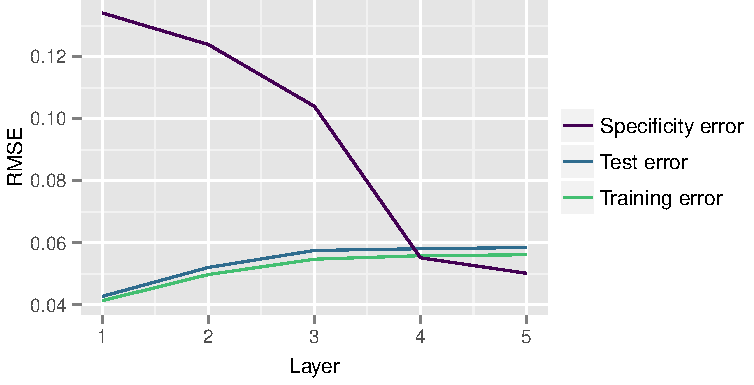
\includegraphics[width=0.8\textwidth]{figures/genspe}

\caption[Generalizability vs. specificity of a DBN for different numbers of
layers]{Generalizability vs. specificity of a DBN for different numbers of
layers. The similarity of the reconstruction errors between the training and
test images indicates that no overfitting occurs. The opposite slopes of the reconstruction errors and error of generated images (specificity error)
indicates a trade-off between generalizability vs. specificity in the earlier
phases of training, but the low errors at layer 5 indicate that the method is
both generalizable and specific.}
\label{fig:genspe}
\end{figure}

\begin{figure}[tb!]
\centering
% \includegraphics[width=0.5\textwidth, trim=0 0em 0 0]
%   {figures/MICCAI2013_sampled2d}
  
\begin{tikzpicture}
\tikzstyle{every node}+=[font=\small]
\node[inner sep=6pt] (manifold)
{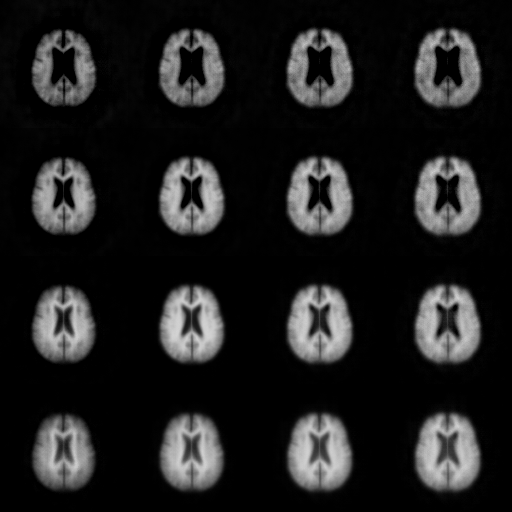
\includegraphics[width=0.5\textwidth]{figures/MICCAI2013_sampled2d}};

\draw[->] (manifold.south west)--node[below=5pt,inner sep=0] {$M_1$}
(manifold.south east);
\draw[->] (manifold.south west)--node[above=5pt,sloped,inner sep=0] {$M_2$}
(manifold.north west);

\end{tikzpicture}

\caption[Axial slices from generated volumes from the manifold]{Axial slices
from generated volumes from the manifold. An increase of the first and second manifold dimension visually correlates with an increase in
brain and ventricle size, respectively.}
\label{fig:generated}
\end{figure}

\subsubsection{Visualization of the Learned Manifold}

\ref{fig:generated} shows axial slices of 16 volumes sampled at the grid points
of a 2D regular grid in manifold space. Volumes sampled along the first manifold
dimension $M_1$ (from left to right) appear to increase in brain size, and the
images sampled along the second manifold dimension $M_2$ (from bottom to top)
appear to increase in ventricle size. \ref{fig:scatter} shows an axial slice of
each image of the training set plotted against its manifold coordinates.
Consistent with images sampled from the manifold, an increase in ventricle size,
which is indicative of brain atrophy (a hallmark of AD), visually correlates
with an increase of the second manifold coordinate. The AD/normal status is
indicated by the frame color of each image. The vertical separation between AD
and normals suggests that the second manifold coordinate is potentially of
practical use in differentiating between AD and normal.

\begin{figure}[tb!] \centering
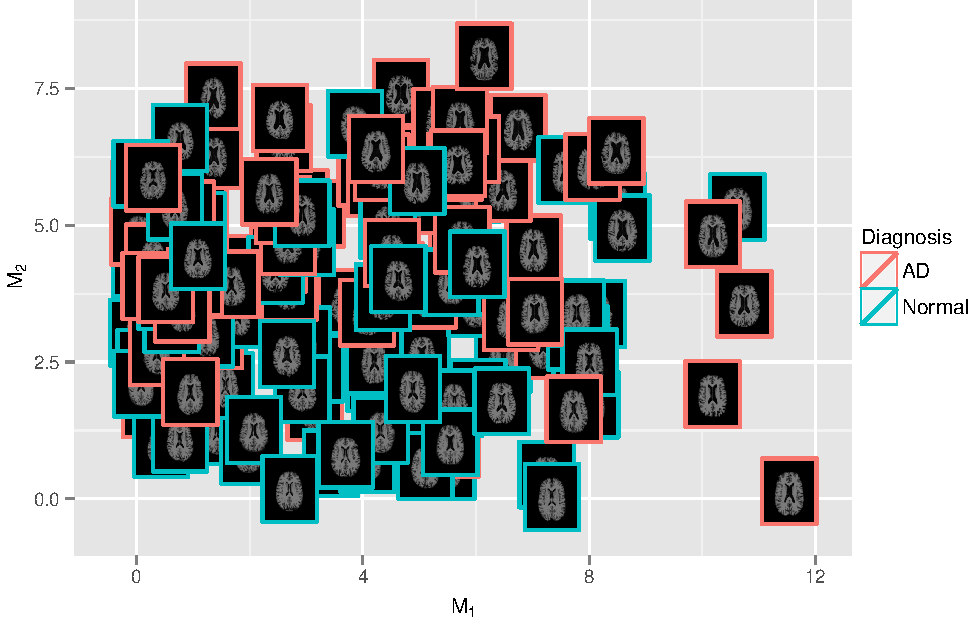
\includegraphics[width=\textwidth]{figures/scatterimage}
\caption[Axial slices of volumes from the training set plotted against their
manifold coordinates]{Axial slices of volumes from the training set plotted
against their manifold coordinates. The brains with larger ventricles, indicative of atrophy,
are mostly at the top, which is also where most of the AD patients are.}
\label{fig:scatter}
\end{figure}

\subsubsection{Correlations with Clinical Parameters}

To evaluate the potential of the manifold coordinates to reveal or predict
clinically relevant information, we have calculated the Pearson correlation $r$
of demographic parameters (age, gender) and disease parameters (MMSE score,
AD/normal status) with the manifold coordinates ($M_1$ and $M_2$). The results
of the correlation tests are summarized in \ref{tab:corr}. Age, MMSE and
AD/normal status show highly significant correlations with $M_2$ ($p$-values
between \num{9.85e-9} and \num{3.53e-7}), which makes intuitive sense because
$M_2$ visually correlates with ventricle size. The first manifold coordinate
correlates strongest with gender ($p\text{-value} = \num{8.24e-9}$), which also
makes sense in terms of the general difference in size between male and female.
The strength and significance of the correlations demonstrate the potential of
deep learning of brain images for classification and prediction of disease
status.

\begin{table}[tb]
\small
\centering
\caption[Pearson correlation of demographic and clinical parameters with
manifold coordinates]{Pearson correlation $r$ of demographic and
clinical parameters with manifold coordinates ($M_1$, $M_2$). The stronger
correlation in each column is highlighted in bold.}
\sisetup{
  round-mode = places,
  round-precision = 2,
  exponent-product = \cdot,
  detect-weight=true,detect-inline-weight=math,
  tight-spacing = true
}%

\begin{tabular}{l*{4}{@{\hspace{15pt}}cc}}
\toprule
& \multicolumn{2}{c}{Age} & \multicolumn{2}{c}{Gender} &
\multicolumn{2}{c}{MMSE} & \multicolumn{2}{c}{AD/Normal Status} \\
& $r$ & $p$-value & $r$ & $p$-value & $r$ & $p$-value
& $r$ & $p$-value \\
\midrule
% V1
$M_1$ &
\num{-0.1734} & \num{0.03378} &
\textbf{\num{0.4490381}} & \textbf{\num{8.239e-09}} &
\num{0.0116499} & \num{0.8875} &
\num{-0.03231144} & \num{0.6947} \\
% V2
$M_2$ &
\textbf{\num{0.4469}} & \textbf{\num{9.848e-09}} &
\num{0.1860143} & \num{0.02266} &
\textbf{\num{-0.4015518}} & \textbf{\num{3.527e-07}} &
\textbf{\num{0.4127084}} & \textbf{\num{1.536e-07}} \\
\bottomrule
\end{tabular}
\label{tab:corr}
\end{table}

\section[Variability of morphology and lesion distribution]{Variability of
Morphology and Lesion Distribution}

In this section, we present a new method for modeling the variability in brain
morphology and lesion distribution in a large set of MRIs of MS patients.
Similar to our previous work on modeling the manifold of brain MRIs of AD and
healthy subjects, our method is built using a DBN \citep{hinton2006b}, a layered
network whose parameters can be learned from training images. However, a
difference to the previous approach is that the DBN is trained on deformation
fields and lesions masks, instead of brain MRIs, in order to focus on the
learning of the variability in brain morphology and lesion distribution, without
the confounding influence of intensity variations. An advantage of DBNs over
other manifold learning methods is that it does not require a prebuilt proximity
graph, which is particularly beneficial for modeling lesions, because the
spareness and randomness of MS lesions make defining a suitable distance measure
challenging and potentially biasing. Instead, the DBN approach assumes that a
particular lesion configuration is a sample from an unknown distribution of
lesion configurations that can be parameterized by a relatively small set of
lesion distribution parameters. We model morphological and lesion variability
with two individual DBNs, then form a joint model by replacing the individual
top network layers with a new layer that joins both DBNs, similarly to the work
on the joint modeling of auditory and visual signals for speech recognition
\citep{ngiam2011}. Our results show that this model can automatically discover
the classic patterns of MS pathology, as well as more subtle ones, and that the
distribution parameters computed are found to have strong relationships to MS
clinical scores.

% Short overview. New data. Deformation fields directly and lesion masks for MS.
% Motivation for that: correspondence but without eliminating variability in
% morphology. Why use deep learning and not another method for that?

\subsection[Data sets and preprocessing]{Data Sets and Preprocessing}

The proposed method was evaluated on a data set from an MS clinical trial of 474
secondary progressive MS patients. For each subject, the data set contains one
\gls{t1w}, \gls{t2w}, and \gls{pdw} MRI with a resolution of \num{256x256x50}
voxels and a voxel size of \SI{0.937x0.937x3.000}{\milli\meter}. The main
preprocessing steps included rigid registration, brain extraction, intensity
normalization, and background cropping.

\begin{figure}[tb]
\centering
\begin{tikzpicture}[scale=0.75]
\tikzstyle{every node}=[font=\sffamily\small, inner sep=3pt, align=center]
\tikzstyle{every pin}=[align=center,fill=white]
\tikzstyle{dbnlabel}=[font=\sffamily]
         
% Deformation field
        
\node[dbnlabel, rotate=90] at (-1.5,2.25) {Morphology DBN};
        
\begin{scope}[xshift=-20pt,yslant=0.63,xscale=0.4]

\node[transform shape,pin={[pin
distance=8]125:Displacement\\
field $u$}] (field) at (2,2)
{\includegraphics[width=4cm]{figures/deformation2.png}};

% \node[pin={[pin distance=0.6,overlay]93:Displacement\\
% field $u$}] at ($(field.north west)!0.1!(field.north east)$) {};

\end{scope}
         
% 3-channel input

\foreach \x in {0, 10, 20} {
\begin{scope}[xshift=\x pt]
%\ifnum\x=0
%\path
%\else
\draw[fill=white, fill opacity=0.75]
%\fi
  (0,0) coordinate(A\x) -- ++(90:4) coordinate (B\x) -- ++(30:2) coordinate
  (C\x) -- ++(-90:4) -- cycle;
  

% \begin{scope}[xshift=-50pt,yslant=0.63,xscale=0.4]  
% \node[transform shape,inner sep=0pt] at (2,2)
%   {\includegraphics[width=4cm]{deformation2.png}};
% \end{scope}
  
\draw (0,3)
   ++(30:0.25) \ifnum\x=20 coordinate (a1) \else -- +(0:10pt) +(0:0) \fi
-- ++(90:0.5)  \ifnum\x=20 coordinate (b1) \else -- +(0:10pt) +(0:0) \fi
-- ++(30:0.25) \ifnum\x=20 coordinate (c1) \else -- +(0:10pt) +(0:0) \fi
-- ++(-90:0.5) \ifnum\x=20 coordinate (d1) \else -- +(0:10pt) +(0:0) \fi
-- ++(210:0.25);
\end{scope}
}

%\node[below=4pt,xshift=-3pt] at (A0)  {$u_x$};
%\node[below=4pt] at (A10) {$u_y$};
%\node[below=4pt,xshift=3pt] at (A20) {$u_z$};

\node[pin={[pin distance=5pt]260:$u_x$}] at (A0)  {};
\node[pin={[pin distance=5pt]270:$u_y$}] at (A10)  {};
\node[pin={[pin distance=5pt]290:$u_z$}] at (A20)  {};

% Transition

\draw ($(a1)!0.5!(c1)$) ++(55pt,-5pt) coordinate (e1);
\draw (a1) -- (e1);
\draw (b1) -- (e1);
\draw (c1) --node[pin={[pin distance=1cm]40:Strided\\ convolution}] {} (e1);
\draw (d1) -- (e1);

% First layer hidden units

\foreach \x in {80,85,90,95,100,105} {
\begin{scope}[xshift=\x pt,yshift=1.5cm,scale=0.5]
\draw[fill=white, fill opacity=0.75]
  (0,0) coordinate(A\x) -- ++(90:4) coordinate (B\x) -- ++(30:2) coordinate
  (C\x) -- ++(-90:4) coordinate(D\x) -- cycle;
   
\draw (0,2.5)
   ++(30:0.25) \ifnum\x=105 coordinate (a2) \else -- +(0:10pt) +(0:0) \fi
-- ++(90:1)    \ifnum\x=105 coordinate (b2) \else -- +(0:10pt) +(0:0) \fi
-- ++(30:0.5)  \ifnum\x=105 coordinate (c2) \else -- +(0:10pt) +(0:0) \fi
-- ++(-90:1)   \ifnum\x=105 coordinate (d2) \else -- +(0:10pt) +(0:0) \fi
-- ++(210:0.5);
\end{scope}
}

\draw[decorate,decoration={brace,raise=20pt}] (B0|-C0) --node[above=25pt]
{Strided convolutional RBM} (C105|-C0);

\draw[decorate,decoration={brace,raise=4pt,mirror}]
%(A80) --node[below=8pt] {$N = 32$} (A80-|D105);
(A80) --node[below=8pt] {$N = 32$} (A80-|D105);

\draw ($(a2)!0.5!(c2)$) ++(0:38pt) coordinate (e2);
\draw (a2) -- (e2);
\draw (b2) -- (e2);
\draw (c2) -- (e2);
\draw (d2) -- (e2);

% Second layer hidden units

\foreach \x in {145, 150, ..., 175, 180} {
\begin{scope}[xshift=\x pt,yshift=2.25cm,scale=0.25]
\draw[fill=white, fill opacity=0.75]
  (0,0) coordinate(A\x) -- ++(90:4) coordinate (B\x) -- ++(30:2) coordinate
  (C\x) -- ++(-90:4) coordinate(D\x) -- cycle;
\draw (0,1.75)
   ++(30:0.25) \ifnum\x=180 coordinate (a3) \else -- +(0:20pt) +(0:0) \fi
-- ++(90:2)    \ifnum\x=180 coordinate (b3) \else -- +(0:20pt) +(0:0) \fi
-- ++(30:1)    \ifnum\x=180 coordinate (c3) \else -- +(0:20pt) +(0:0) \fi
-- ++(-90:2)   \ifnum\x=180 coordinate (d3) \else -- +(0:20pt) +(0:0) \fi
-- ++(210:1);
\end{scope}
}

\draw[decorate,decoration={brace,raise=4pt,mirror}]
(A145) --node[below=8pt] {$N = 64$} (A145-|D180);

\draw ($(a3)!0.5!(c3)$) ++(0:18pt) coordinate (e3);
\draw (a3) -- (e3);
\draw (b3) -- (e3);
\draw (c3) -- (e3);
\draw (d3) -- (e3);

% Third layer hidden units

\foreach \x in {200, 205, ..., 240} {
\begin{scope}[xshift=\x pt,yshift=2.625cm,scale=0.125]
\draw[fill=white, fill opacity=0.75]
  (0,0) coordinate(A\x) -- ++(90:4) coordinate (B\x) -- ++(30:2) coordinate
  (C\x) -- ++(-90:4) coordinate(D\x) -- cycle;
\end{scope}
}

% Forth layer visible units (dense)

\begin{scope}[xshift=280pt, yshift=2.75cm]
\foreach \x/\y in {0/-2, 1/-1.5, 2/-1, 3/-0.5, 4/0, 5/0.5, 6/1, 7/1.5, 8/2} {
  \node[circle, draw] (v\x) at (0,\y) {};
}
\end{scope}

\draw[shorten >=10pt,shorten <=10pt,dashed] (A240)--(v0.south west);
\draw[shorten >=10pt,shorten <=10pt,dashed] (A240|-C240)--
node[label=120:Vectorize\\ hidden units] {} (v8.north west);

\draw[decorate,decoration={brace,raise=4pt,mirror}]
(A200) --node[below=8pt,fill=white] {$N = 32$} (A200-|D240);

%\node[rotate=90,fill=white,align=center] at(270pt,2.75cm) {Serialize\\ hidden
%units};

% Forth layer hidden units (dense)

\begin{scope}[xshift=320pt, yshift=2.75cm]
\foreach \x/\y in {0/-1, 1/-0.5, 2/0, 3/0.5, 4/1} {
  \node[circle, draw] (h\x) at (0,\y) {};
}
\end{scope}

\foreach \x in {0, ..., 8} {
  \foreach \y in {0, ..., 4} {
    \draw[very thin] (v\x)--(h\y);
  }
}

\draw[decorate,decoration={brace,raise=20pt}] (v8.west|-C0)
--node[above=25pt] {Dense RBM} (h0.east|-C0);

% Fifth layer hidden units (distribution parameters)

\begin{scope}[xshift=360pt, yshift=2.75cm]
\foreach \x/\y in {1/0.25, 2/-0.25} {
  \node[circle, draw, label=0:$D_\x$] (D\x) at (0,\y) {};
}
\end{scope}

\foreach \x in {0, ..., 4} {
  \foreach \y in {1,2} {
    \draw[very thin] (h\x)--(D\y);
  }
}

% \draw[decorate,decoration={brace,raise=22pt}]
% (D1.north-|D1.east) --node[above,sloped] {Deformation\\ parameters}
% (D2.south-|D2.east);

%%%%%%%%%%%%%%%%%%%%%
% Lesion Model
%%%%%%%%%%%%%%%%%%%%%

\begin{scope}[yshift=-6cm]

\node[dbnlabel, rotate=90] at (-1.5,2.25) {Lesion DBN};

\begin{scope}[xshift=-25pt,yslant=0.63,xscale=0.4] 
\node[transform shape,pin={[pin distance=15]140:Lesion\\
mask $l$}] at (2,2)
  {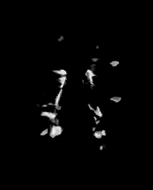
\includegraphics[height=4cm]{figures/lesions.png}};
\end{scope}

% 1-channel input

\foreach \x in {20} {
\begin{scope}[xshift=\x pt]
\draw[fill=white, fill opacity=0.75]
  (0,0) coordinate(A\x) -- ++(90:4) coordinate (B\x) -- ++(30:2) coordinate
  (C\x) -- ++(-90:4) coordinate (D\x) -- cycle;
  
\draw (0,3)
   ++(30:0.25) \ifnum\x=20 coordinate (a1) \else -- +(0:10pt) +(0:0) \fi
-- ++(90:0.5)  \ifnum\x=20 coordinate (b1) \else -- +(0:10pt) +(0:0) \fi
-- ++(30:0.25) \ifnum\x=20 coordinate (c1) \else -- +(0:10pt) +(0:0) \fi
-- ++(-90:0.5) \ifnum\x=20 coordinate (d1) \else -- +(0:10pt) +(0:0) \fi
-- ++(210:0.25);
\end{scope}
}

\node[pin=30:Visible\\ units] at ($(C20)!0.25!(D20)$) {};

% Transition

\draw ($(a1)!0.5!(c1)$) ++(55pt,-5pt) coordinate (e1);
\draw (a1) -- (e1);
\draw (b1) -- (e1);
\draw (c1) -- (e1);
\draw (d1) -- (e1);

% First layer hidden units

\foreach \x in {80,85,90,95,100,105} {
\begin{scope}[xshift=\x pt,yshift=1.5cm,scale=0.5]
\draw[fill=white, fill opacity=0.75]
  (0,0) coordinate(A\x) -- ++(90:4) coordinate (B\x) -- ++(30:2) coordinate
  (C\x) -- ++(-90:4) coordinate(D\x) -- cycle;
   
\draw (0,2.5)
   ++(30:0.25) \ifnum\x=105 coordinate (a2) \else -- +(0:10pt) +(0:0) \fi
-- ++(90:1)    \ifnum\x=105 coordinate (b2) \else -- +(0:10pt) +(0:0) \fi
-- ++(30:0.5)  \ifnum\x=105 coordinate (c2) \else -- +(0:10pt) +(0:0) \fi
-- ++(-90:1)   \ifnum\x=105 coordinate (d2) \else -- +(0:10pt) +(0:0) \fi
-- ++(210:0.5);
\end{scope}
}

\draw[decorate,decoration={brace,raise=4pt,mirror}]
%(A80) --node[below=8pt] {$N = 32$} (A80-|D105);
(A80) --node[below=8pt] {$N = 32$} (A80-|D105);

\draw ($(a2)!0.5!(c2)$) ++(0:38pt) coordinate (e2);
\draw (a2) -- (e2);
\draw (b2) -- (e2);
\draw (c2) -- (e2);
\draw (d2) -- (e2);

\node[pin=30:Hidden\\ units] at ($(C105)!0.2!(D105)$) {};

% Second layer hidden units

\foreach \x in {145, 150, ..., 175, 180} {
\begin{scope}[xshift=\x pt,yshift=2.25cm,scale=0.25]
\draw[fill=white, fill opacity=0.75]
  (0,0) coordinate(A\x) -- ++(90:4) coordinate (B\x) -- ++(30:2) coordinate
  (C\x) -- ++(-90:4) coordinate(D\x) -- cycle;
\draw (0,1.75)
   ++(30:0.25) \ifnum\x=180 coordinate (a3) \else -- +(0:20pt) +(0:0) \fi
-- ++(90:2)    \ifnum\x=180 coordinate (b3) \else -- +(0:20pt) +(0:0) \fi
-- ++(30:1)    \ifnum\x=180 coordinate (c3) \else -- +(0:20pt) +(0:0) \fi
-- ++(-90:2)   \ifnum\x=180 coordinate (d3) \else -- +(0:20pt) +(0:0) \fi
-- ++(210:1);
\end{scope}
}

\draw[decorate,decoration={brace,raise=4pt,mirror}]
(A145) --node[below=8pt] {$N = 64$} (A145-|D180);

\draw ($(a3)!0.5!(c3)$) ++(0:18pt) coordinate (e3);
\draw (a3) -- (e3);
\draw (b3) -- (e3);
\draw (c3) -- (e3);
\draw (d3) -- (e3);

% Third layer hidden units

\foreach \x in {200, 205, ..., 240} {
\begin{scope}[xshift=\x pt,yshift=2.625cm,scale=0.125]
\draw[fill=white, fill opacity=0.75]
  (0,0) coordinate(A\x) -- ++(90:4) coordinate (B\x) -- ++(30:2) coordinate
  (C\x) -- ++(-90:4) coordinate(D\x) -- cycle;
\end{scope}
}

%\node[rotate=90] at(270pt,2.75cm) {Serialize hidden units};

% Forth layer visible units (dense)

\begin{scope}[xshift=280pt, yshift=2.75cm]
\foreach \x/\y in {0/-2, 1/-1.5, 2/-1, 3/-0.5, 4/0, 5/0.5, 6/1, 7/1.5, 8/2} {
  \node[circle, draw] (V\x) at (0,\y) {};
}
\end{scope}

\draw[shorten >=10pt,shorten <=10pt,dashed] (A240)--(V0.south west);
\draw[shorten >=10pt,shorten <=10pt,dashed] (A240|-C240)--
%node[label=120:Vectorize\\ hidden units] {}
(V8.north west);

\draw[decorate,decoration={brace,raise=4pt,mirror}]
(A200) --node[below=8pt,fill=white] {$N = 32$} (A200-|D240);

%\node[rotate=90,fill=white,align=center] at(270pt,2.75cm) {Serialize\\ hidden
%units};

% Forth layer hidden units (dense)

\begin{scope}[xshift=320pt, yshift=2.75cm]
\foreach \x/\y in {0/-1, 1/-0.5, 2/0, 3/0.5, 4/1} {
  \node[circle, draw] (H\x) at (0,\y) {};
}
\end{scope}

\foreach \x in {0, ..., 8} {
  \foreach \y in {0, ..., 4} {
    \draw[very thin] (V\x)--(H\y);
  }
}

% Fifth layer hidden units (distribution parameters)

\begin{scope}[xshift=360pt, yshift=2.75cm]
\foreach \x/\y in {1/0.25, 2/-0.25} {
  \node[circle, draw, label=0:$L_\x$] (L\x) at (0,\y) {};
}
\end{scope}

\foreach \x in {0, ..., 4} {
  \foreach \y in {1,2} {
    \draw[very thin] (H\x)--(L\y);
  }
}
\end{scope}

%%%%%%%%%%%%%%
% Joint layer
%%%%%%%%%%%%%%

% yshift = 2.75 - 6/2 = -0.25

\begin{scope}[xshift=380pt, yshift=-0.25cm]
\foreach \x/\y in {1/-0.75, 2/-0.25, 3/0.25, 4/0.75} {
  \node[circle, draw, label=0:$J_\x$] (J\x) at (0,\y)
  {}; }
\end{scope}

\foreach \x in {0, ..., 4} {
  \foreach \y in {1, ..., 4} {
    \draw[very thin] (h\x)--(J\y);
    \draw[very thin] (H\x)--(J\y);
  }
}

\node[yshift=-15pt, fill=white, inner sep=3pt] at (h0) {$N = 16$};

\draw[decorate,decoration={brace,raise=30pt,mirror}] (V0.south-|J1)
--node[dbnlabel, below=35pt, sloped] {Joint DBN} (v8.north-|J1);

\end{tikzpicture}
\caption{DBN models used for discovering patterns.}
\label{fig:msdbnmodel}
\end{figure}

\subsection{Method}

\glsunset{icbm}\glsunset{mni}
Our proposed model for pattern discovery is illustrated in \ref{fig:msdbnmodel}
and consists of three main components (a) a model that aims to find patterns of
morphological changes in deformation fields (top pathway), (b) a model that aims
to find patterns in the spatial distribution of lesions (bottom pathway), and
(c) a joint model that aims to find concurring deformation and lesion
distribution patterns (combined pathways).

\subsubsection{Morphology Model}

The morphology model is learned from a set of displacement fields that are
calculated via non-rigid registration from a set of T1w brain MRIs $D \subset
I$, $I = \{I_n \mid I_n\colon\Omega \mapsto \R$\}, $\Omega \subset \R^3$ and the
\gls{icbm} 152 nonlinear atlas template image \citep{fonov2011}. First, all
images of the training set are aligned to \gls{mni} space by a 9
degree-of-freedom registration using the \gls{flirt} \citep{jenkinson2002}. Then
for each image $I_n \in D$, the displacement field $u_n$, $u\colon \Omega
\mapsto \R^3$, that describes the non-rigid transformation from template
coordinates to image coordinates is calculated using the \gls{fnirt}
\citep{andersson2007}, where the displacement field $u_n$ is represented by a
\num{40x48x22} grid of 3D displacement vectors. We assume that the displacement
fields $u_n$ are samples from an unknown distribution $p(u \mid D_1, \dotsc)$
that can be parameterized by far fewer parameters than the dimensionality of the
fields themselves. In practice, the user typically selects the number of
parameters to represent the data being explored. The task of finding patterns is
to discover the underlying probability density function $p(u \mid D_1, \dotsc)$,
where the parameters $(D_1,\dotsc)^T$ represent the patterns of variability of
the displacement field distribution. This allows us to compare the morphology of
two brains at a very high level in terms of the distribution parameters of their
displacement fields $u_1$ and $u_2$ given by $\E[D_1,\dotsc \mid u_1]$ and
$\E[D_1,\dotsc \mid u_2]$. Furthermore, we can visualize the modes of
morphological variability of MS brain images, by sampling the space of
displacement fields spanned by $(D_1, \dotsc)^T$ by calculating the expectation
$\E[u \mid D_1, \dotsc]$ for a range of values for $(D_1, \dotsc)^T$.

The probability density function $p(u)$ is modeled by a \gls{dbn}
\citep{hinton2006b}. The first RBM layer receives the displacement fields of a
training set as input and reduces the dimensionality of each field by
discovering patterns of similarity that are common within groups of displacement
fields. Each subsequent RBM receives the hidden unit activations of the previous
RBM as input, thus learning successively more complex and abstract patterns from
the training data. In particular, we use a DBN with three sconvRBMs and two
dense RBMs as described in \ref{sec:general_arch}. Compared to other more
commonly used convolution-based RBMs \citep{lee2009}, an advantage of sconvRBMs
is that inference is invertible, which allows the reconstruction of the visible
units from the hidden unit activations. In our application, this would allow for
the reconstruction of deformation fields from distribution parameters.

\begin{table}[t!]
\caption[Training parameters of the morphology DBN, lesion DBN, and joint
DBN]{Training parameters of the morphology DBN, lesion DBN, and joint DBN.
The visible units of the joint DBN are composed of the concatenated hidden
units of the first dense RBMs of the morphology and lesion DBNs.}
\label{tab:msdbn}
\centering
\small
\begin{tabular}{llccc}
\toprule
Layer & Parameter & Morphology DBN & Lesion DBN & Joint DBN \\
\midrule
Input     & Image size  & \num{40x48x22x3}  & \num{160x192x56x1} & --- \\
\addlinespace
sconvRBM1 & Stride size & \num{2x2x1}       & \num{4x4x2} & --- \\
          & Filter size & \num{10x10x7}     & \num{20x20x10} & --- \\
          & Filters     & 32                & 32 & --- \\
          & Output size & \num{16x20x16x32} & \num{36x44x24x32} & --- \\
\addlinespace
sconvRBM2 & Stride size & \num{2x2x2}       & \num{2x2x2} & --- \\
          & Filter size & \num{10x10x10}    & \num{14x14x10} & --- \\
          & Filters     & \num{64}          & \num{64} & --- \\
          & Output size & \num{4x6x4x64}    & \num{12x16x8x64} & --- \\
\addlinespace
sconvRBM3 & Stride size & \num{1x1x1}       & \num{2x2x2} & --- \\
          & Filter size & \num{3x5x3}       & \num{10x14x6} & --- \\
          & Filters     & 32                & 64 & --- \\
          & Output size & \num{2x2x2x32}    & \num{2x2x2x64} & --- \\
\addlinespace
RBM1      & Visible units & 256 & 512 & --- \\
          & Hidden units  &  16 & 16 & ---  \\
\addlinespace
RBM2      & Visible units & 16  & 16 & 32 \\
          & Hidden units  &  2  &  2 &  4 \\
\bottomrule
\end{tabular}
\end{table}

The parameters of the morphology DBN are summarized in \ref{tab:msdbn}. In
contrast to the DBN used to learn the manifold of brain MRIs of AD and healthy
subjects, we use valid convolutions for the sconvRBMs, because they allow a much
faster reduction of the dimensionality, especially for layers two and three,
where the image sizes are relatively small compared to the filter sizes. This
allows for a greater reduction of dimensionality within the sconvRBM layers, and
consequently for a more gradual reduction of the number of hidden units during
the transition of sconvRBMs to dense RBMs. To roughly compensate for the
anisotropic voxel size of the input images and corresponding deformation
fields, we chose an anisotropic filter and stride size of \num{10x10x7} and
\num{2x2x1}, respectively. After three sconvRBMs, the size of a deformation
field is reduced to \num{2x2x2x32} and small enough for RBMs.

Once the weights and bias terms of the DBN have been learned
from training data, we can use the model for inference. Let
$\vect{v}_{\text{d},1}, \dotsc, \vect{v}_{\text{d},5}$, $\vect{h}_{\text{d},1},
\dotsc, \vect{h}_{\text{d},5}$, and $\thetas_{\text{d},1}, \dotsc,
\thetas_{\text{d},5}$ denote the visible units, hidden units, and parameters,
respectively, of each RBM of the morphology DBN. Then, for a given displacement
field $u_n$, we can calculate the parameters $(D_1, \dotsc)^T$ of $u_n \sim p(u
\mid D_1, \dotsc)$ with
\begin{align} 
(D_1, \dotsc)^T &= \E[D_1, \dotsc \mid u_n] = \E[\vect{h} \mid
\vect{v}_{\text{d},5}, \thetas_{\text{d},5}] \\
\vect{v}_{\text{d},i+1} &= \E[\vect{h} \mid \vect{v}_{\text{d},i},
\thetas_{\text{d},i}]
\end{align}
where $i \in [1,4]$ and $\vect{v}_{\text{d},1} = u_n$. Inversely, the mean
displacement field $\bar{u}$ given the distribution parameters can be calculated
by
\begin{align}
\bar{u} &= \E[u \mid D_1, \dotsc] = \E[\vect{v} \mid \vect{h}_{\text{d},1},
\thetas_{\text{d},1}] \\
\vect{h}_{\text{d},i} &= \E[\vect{v} \mid \vect{h}_{\text{d},i+1},
\thetas_{\text{d},i+1}]
\end{align}
where $i \in [1,4]$ and $\vect{h}_{\text{d},5} = (D_1,\dotsc)^T$.

\subsubsection{Lesion Model}

The input into our lesion model is a set of 3D binary lesion masks $l_n \in I$,
which have been created from T2w and PDw MRIs by experts using a semi-automatic
method. All lesion masks are spatially aligned to MNI space using the
transformations as calculated for the corresponding T1w images. Analogous to the
morphology model, we assume that lesion masks $l_n$ are samples from an unknown
distribution $l_n \sim p(l \mid L_1, \dotsc)$ that can be parameterized by only
relatively few parameters $(L_1, \dotsc)^T$. The task of finding lesion patterns
is to discover the underlying probability density function $p(l \mid L_1,
\dotsc)$, where the parameters $(L_1, \dotsc)^T$ represent patterns of
variability of MS lesions. Similar to the morphology DBN, the lesion DBN
consists of three sconvRBMs and two dense RBMs, whose parameters are summarized
in \ref{tab:msdbn}. For the first layer, we chose an anisotropic stride size of
\num{4x4x2}, to roughly compensate for the anisotropic voxel size of the input
images. A limiting factor for the choice of parameters is the amount of
available GPU memory. Due to the much higher resolution of the lesion masks
compared to the deformation fields, we increased the stride size compared to the
morphology DBN in order to reduce the required amount of memory for storing the
hidden units of the first layer and visible units of the second layer. Choosing
a stride size of \num{4x4x2} reduces the size of one channel by a factor of
roughly 32, which allows the use of 32 filters, while keeping the amount of
memory required to train the second layer roughly equal compared to the first
layer. To account for the sparse activation of MS lesion masks, we constrain the
filter learning process to a pre-defined ROI, which was chosen to contain all
white matter lesions from the training set. Similarly to the morphology model,
for a trained lesion DBN and a given lesion mask $l_n$, we can calculate the
parameters $(L_1,\dotsc)^T$ of $l_n \sim p(l\mid L_1,\dotsc)$ by
\begin{align} 
(L_1, \dotsc)^T &= \E[L_1, \dotsc \mid l_n] = \E[\vect{h} \mid
\vect{v}_{\text{l},5}, \thetas_{\text{l},5}] \\
\vect{v}_{\text{l},i+1} &= \E[\vect{h} \mid \vect{v}_{\text{l},i},
\thetas_{\text{l},i}]
\end{align}
where $i \in [1,4]$ and $\vect{v}_{\text{l},1} = l_n$. Likewise, the mean lesion
configuration $\bar{l}$ given the distribution parameters $(L_1,\dotsc)^T$ can
be calculated by
\begin{align}
\bar{l} &= \E[l \mid L_1, \dotsc] = \E[\vect{v} \mid \vect{h}_{\text{l},1},
\thetas_{\text{l},1}] \\
\vect{h}_{\text{l},i} &= \E[\vect{v} \mid \vect{h}_{\text{l},i+1},
\thetas_{\text{l},i+1}]
\end{align}
where $\vect{v}_{\text{l},1}, \dotsc, \vect{v}_{\text{l},5}$,
$\vect{h}_{\text{l},1}, \dotsc, \vect{h}_{\text{l},5}$, and
$\thetas_{\text{l},1}, \dotsc, \thetas_{\text{l},5}$ denote the visible units,
hidden units, and parameters of each RBM of the lesion DBN, respectively, $i \in
[1,4]$, and $\vect{h}_{\text{l},5} = (L_1,\dotsc)^T$.

\subsubsection{Joint Model}

To discover concurring patterns of morphology and lesion distribution, we
combine the morphology DBN and the lesion DBN to form the joint DBN, which
defines the joint distribution $p(u, l \mid J_1, \dotsc)$. The joint DBN
consists of two pathways (see \ref{fig:msdbnmodel}), each corresponding to the
first 4 layers of the morphology and lesion DBNs, respectively, and a 5th RBM
layer with 4 hidden units, which replaces the 5th layer of the individual DBNs
and combines the hidden unit activations of the 4th layer RBMs. That is, the 5th
RBM defines the joint probability $p(\vect{v}_\text{j}, \vect{h}_\text{j} \mid
\thetas_\text{j})$, where the vector $\vect{v}_\text{j}$ contains the
concatenated hidden units of the 4th layer RBMs, $\vect{v}_\text{j} =
(\vect{h}_{\text{d},4}^T, \vect{h}_{\text{l},4}^T)^T$, and $\vect{h}_\text{j} =
(J_1, \dotsc)^T$ are the modes of variability of morphological and lesion
distribution changes.

\subsection{Results}

\subsubsection[Visualization of patterns of variability]{Visualization of
Patterns of Variability}

The invertibility of our model allows the reconstruction of images from the
distribution parameters to visualize the discovered patterns of variability.
\ref{fig:samples}\subref{fig:deformations} shows axial slices from volumes
generated from the 2-parameter morphology model $p(u \mid D_1, D_2)$. To
generate these images, we calculated the mean displacement fields for varying
values of $D_1$ and $D_2$ to span the range of variability represented by the
training set and applied the inverse deformations to the ICBM 152 template
image. The most apparent morphological variability captured by the morphology
model is ventricular enlargement for $D_1$ and overall brain size for $D_2$.
\ref{fig:samples}\subref{fig:lesions} shows axial slices from the mean lesion
configurations $\E[l \mid L_1, L_2]$ for varying lesion distribution parameters.
An increase of $L_2$ visually correlates with an increase of lesions
specifically around the ventricles, whereas an increase of $L_1$ visually
correlates with an increase of lesions in the entire white matter.

\begin{figure}[tb]
\newlength{\subfigwidth}
\setlength{\subfigwidth}{0.27\textwidth}
\centering
\subfloat[Morphology manifold] {
\label{fig:deformations}
\begin{tikzpicture}
\tikzstyle{every node}+=[font=\small]
\node
(manifold){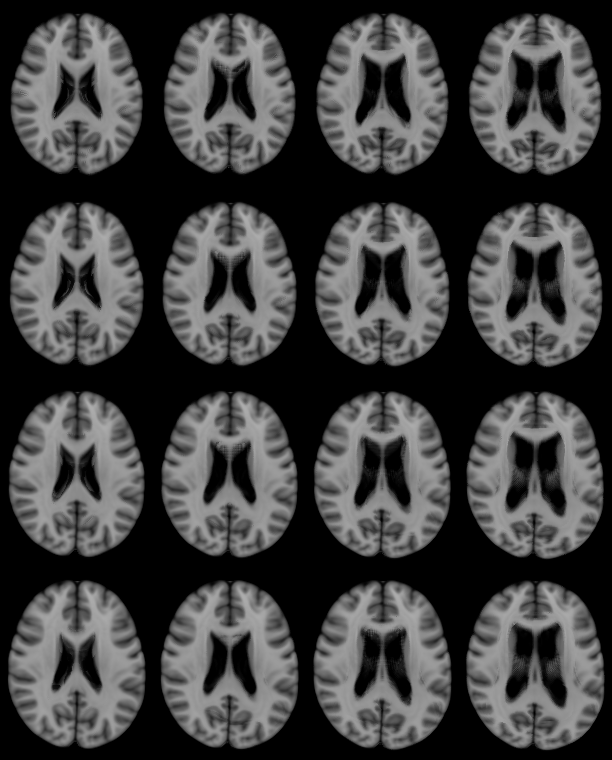
\includegraphics[width=\subfigwidth]{figures/MICCAI2014_warps_t1_dark}};

\draw[->] (manifold.south west)--node[below=5pt,inner sep=0] {$D_1$}
(manifold.south east);
\draw[->] (manifold.south west)--node[above=5pt,sloped,inner sep=0] {$D_2$}
(manifold.north west);

\end{tikzpicture}
}
\subfloat[Lesion manifold] {
\label{fig:lesions}
\begin{tikzpicture}
\tikzstyle{every node}+=[font=\small]
\node
(manifold){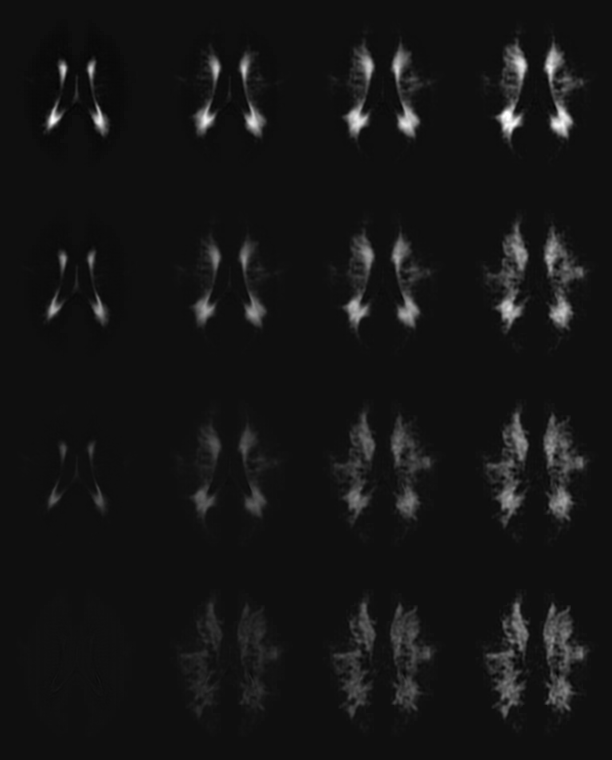
\includegraphics[width=\subfigwidth]{figures/MICCAI2014_p442_d0_full_h16-2}};

\draw[->] (manifold.south west)--node[below=5pt,inner sep=0] {$L_1$}
(manifold.south east);
\draw[->] (manifold.south west)--node[above=5pt,sloped,inner sep=0] {$L_2$}
(manifold.north west);

\end{tikzpicture}
}%
\subfloat[Joint manifold] {
\label{fig:joint}
\begin{tikzpicture}
\tikzstyle{every node}+=[font=\small]

\node[align=left,fill=black,inner sep = 0pt] (manifold1) {
  \mbox{}\\[2pt]
  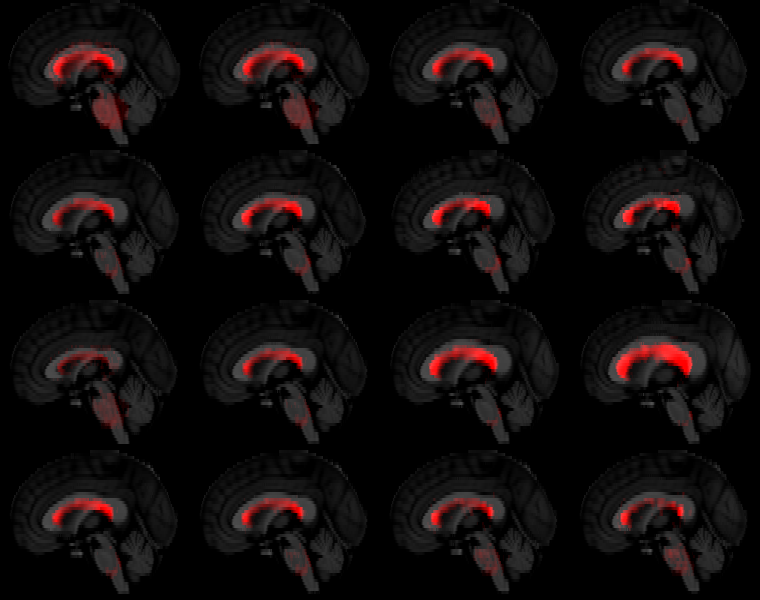
\includegraphics[trim=0 340 0 0,clip,width=\subfigwidth]
    {figures/MICCAI2014_full_rl1_h4_sag}\\[8.5pt]
  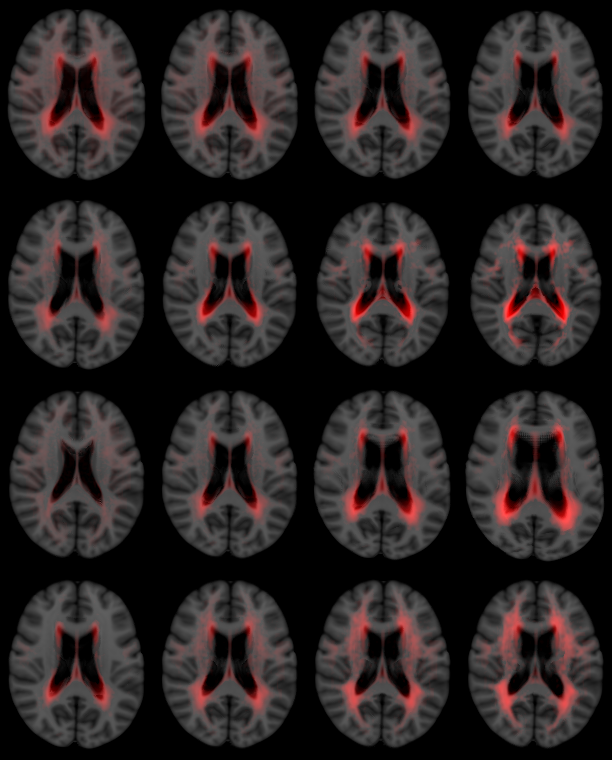
\includegraphics[trim=0 0 0 150,clip,width=\subfigwidth]
    {figures/MICCAI2014_full_rl1_h4}
};
\node[fit=(manifold1)] (manifold) { };

\foreach \x/\y in {0.125/1, 0.375/2, 0.625/3, 0.875/4} {
  \node[left=1pt,inner sep=0pt] at ($(manifold.north west)!\x!(manifold.south
  west)$) {$J_\y$}; }

\draw[->] (manifold.south west)--node[below=5pt,inner sep=0] {$J_x$}
(manifold.south east);

\end{tikzpicture}
} \caption[Slices from generated volumes from the morphology, lesion,
and joint model]{Slices from generated volumes from the (a) morphology, (b)
lesion, and (c) joint model. The morphology model captures ventricular
enlargement ($D_1$) and decrease in brain size ($D_2$) as the main modes of
variation. For the lesion model, $L_1$ captures an increase in lesion load
throughout the WM, while $L_2$ captures primarily periventricular lesion load
variations. The parameters of the joint model capture combinations
of the variability found in the individual models.}
\label{fig:samples}
\end{figure}

To visualize concurring patterns of morphology and lesion distribution, we
sampled images from the joint model $p(u, l \mid J_1, \dotsc, J_4)$ as shown in
\ref{fig:samples}\subref{fig:joint}. The images are deformed template images
with superimposed lesion masks. For each row, we varied only one distribution
parameter and set the remaining parameters to their mean values. Of the four
parameters, $J_3$ visually corresponds most closely to the ``classic''
progression of MS pathology, with an enlargement of the ventricles paired with
an increased periventricular lesion load. The parameters $J_2$ and $J_4$ also
reveal simultaneous morphological and lesion variations that are visible on the
chosen axial slice. For $J_1$, a lesion pattern is not obvious unless the images
are viewed sagittally, which reveals changes in lesion load in the pons.

\subsubsection{Correlations with Clinical Scores}

\begin{table}[tb]
\centering 
%\small

\caption[Pearson correlations of clinical scores with distribution parameters
and imaging biomarkers]{Pearson correlations $r$ of clinical scores with
distribution parameters of the morphology model ($D_1$, $D_2$), lesion model ($L_1$, $L_2$), joint model ($J_1$, $J_2$, $J_3$, $J_4$), normalized brain volume (nBV), and
lesion load (LL). The level of statistical significance is indicated by the
number of asterisks (* $p < 0.05$, ** $p < 0.01$, *** $p < 0.001$).
}

%\NewDocumentCommand{\sym}{m}{#1}

\label{tab:correlations}
\sisetup{
  round-mode = places,
  round-precision = 3,
  exponent-product = \cdot,
  detect-weight=true,
  detect-inline-weight=math,
  tight-spacing = false,
  table-align-text-post = false
}%

\def\tabspace{14pt}

\begin{tabular}{c@{\hspace{\tabspace}}c%
@{\hspace{\tabspace}}S[table-format=2.5]%
@{\hspace{\tabspace}}S[table-format=2.6]
@{\hspace{\tabspace}}S[table-format=2.6]
@{\hspace{\tabspace}}S[table-format=2.6]}
\toprule
 &  & {T25W} & {9-HPT} & {PASAT} & {MSFC} \\
 \midrule
 
\multirow{4}*{\minitab[c]{Individual\\ models}}
 & $D_1$ &
\bfseries -0.128976787246536** & -0.214588136146619*** & -0.282044527648157*** &
-0.314633263656368*** \\
 & $D_2$ & 0.0870255979372807 & 0.115835195120173* & 0.08923208653141 &
0.138616500875685** \\
& $L_1$ & -0.0581629511079419 & -0.231012897586838*** & -0.391822792658197*** &
-0.366992537420278*** \\
& $L_2$ & -0.091057480388512 & \bfseries -0.354478789398171*** &
\bfseries -0.426543205964196*** & \bfseries -0.463860459137063*** \\
\addlinespace
\multirow{4}*{\minitab[c]{Joint\\ model}}
 & $J_1$ & 0.107219513748914* & 0.285812780188632*** & 0.336253511146623*** &
0.378889115681159*** \\
 & $J_2$ & -0.037731447660239 & -0.209982769437628*** & -0.226800472678912***
& -0.255585426983655*** \\
& $J_3$ & \bfseries -0.117780586822506* & \bfseries -0.369169927947271*** &
\bfseries -0.452556545437486*** & \bfseries -0.494130959187706*** \\
& $J_4$ & -0.0491209563011896 & -0.205764640863705*** & -0.382954826511733*** &
-0.345529171963859*** \\
\addlinespace
\multirow{2}*{\minitab[c]{Imaging\\ biomarkers}}
 & nBV & 0.0530068558456253 & 0.143905618421747** & 0.246833144651129***
& 0.234774254053599*** \\
 & LL & -0.073681606595365 & \bfseries -0.286360084620956*** &
\bfseries -0.399646128024074*** & \bfseries -0.406222020153583*** \\
  
 \bottomrule
\end{tabular}

\end{table}

\glsunset{t25w}\glsunset{x9pt}\glsunset{pasat}\glsunset{nbv}\glsunset{ll}
To evaluate the potential of the distribution parameters to reveal clinically
relevant information, we have calculated the Pearson correlation $r$ of the
clinical MS Functional Composite (MSFC) score \citep{fischer1999} and its
components (\glslink{t25w}{Timed 25-Foot Walk, T25W}; \glslink{x9pt}{9-Hole Peg
Test, 9-HPT}; \glslink{pasat}{Paced Auditory Serial Addition Test, PASAT}) with
the distribution parameters and two established MS imaging biomarkers
(\glslink{nbv}{normalized brain volume, nBV}, as calculated by SIENAX
\citep{smith2002} and \glslink{ll}{lesion load, LL}). The results of the
correlation tests are summarized in \ref{tab:correlations}. In the individual
models, all parameters correlate significantly with 9-HPT, PASAT, and MSFC,
except for $D_2$, which did not show a statically significant correlation with
PASAT. The morphology parameter $D_1$ correlates more strongly with these scores
than nBV, as does the lesion parameter $L_2$ than LL. For T25W, $D_1$ shows a
modest but significant correlation while nBV does not. In the joint model, all
parameters correlate significantly with 9-HPT, PASAT, and MSFC, with $J_3$ being
particularly strong. The parameter $J_3$ shows stronger correlations than nBV or
LL for all clinical scores, including a modest significant correlation to T25W,
which is not shown by nBV nor LL. The significant correlation between $J_1$ and
T25W is particularly interesting because the lesion changes modeled by $J_1$
occur in the pons, which is known to be of clinical significance for mobility.
Overall, the learned parameters correlate better than the established imaging
biomarkers.

\begin{figure}[tb]
\centering
\subfloat[Morphological changes] {
\begin{tikzpicture} 
\tikzstyle{every node}=[font=\scriptsize]
\node[align=left,inner sep=0] (images) {
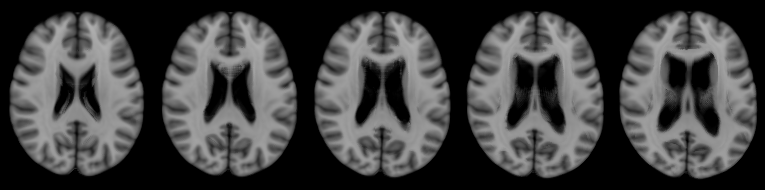
\includegraphics[width=0.47\textwidth]{figures/MICCAI2014_full_rl1_h4_MSFC_nolesion}
\\
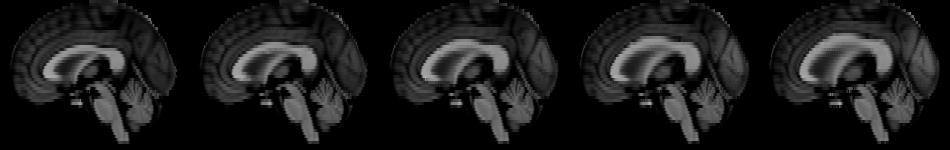
\includegraphics[width=0.47\textwidth]{figures/MICCAI2014_full_rl1_h4_MSFC_sag_nolesion}
};
\foreach \x/\y in {0.1/1.5, 0.3/0, 0.5/-1.5, 0.7/-3, 0.9/-4.5} {
  \node[above=2pt] at ($(images.north west)!\x!(images.north east)$) {$\y$}; }
\end{tikzpicture}
}
\subfloat[Lesion changes] {
\begin{tikzpicture}
\tikzstyle{every node}=[font=\scriptsize] 
\node[align=left,inner sep=0] (images) {
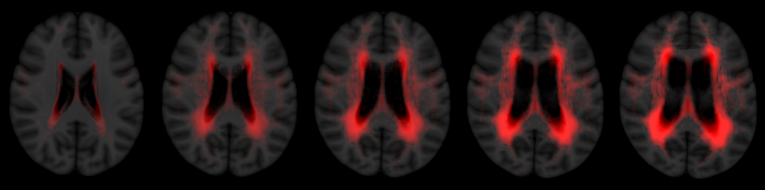
\includegraphics[width=0.47\textwidth]{figures/MICCAI2014_full_rl1_h4_MSFC} \\
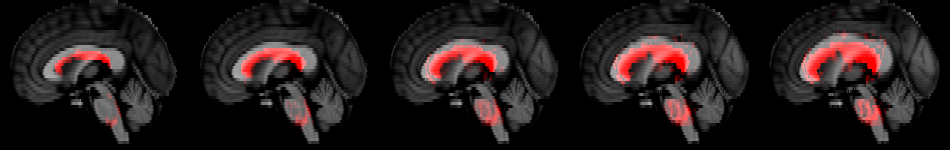
\includegraphics[width=0.47\textwidth]{figures/MICCAI2014_full_rl1_h4_MSFC_sag}
};
\foreach \x/\y in {0.1/1.5, 0.3/0, 0.5/-1.5, 0.7/-3, 0.9/-4.5} {
  \node[above=2pt] at ($(images.north west)!\x!(images.north east)$) {$\y$};
}
\end{tikzpicture}
}
\caption[Axial and mid-sagittal slices of volumes representing the spectrum of
MSFC scores]{Axial (top row) and mid-sagittal (bottom row) slices of volumes
representing the spectrum of MSFC scores from \num{1.5} to \num{-4.5}. A
decrease in MSFC shows the classic pattern of MS pathology.}
\label{fig:msspectrum}
\end{figure}

\subsubsection{Progression of a ``Mean'' SPMS Brain along a Range of MSFC
Scores}

Another benefit of our model is the ability to visualize the progression of a
``mean'' \gls{spms} brain along a range of MSFC scores.
To demonstrate, we trained four independent linear models to predict the
distribution parameters $J_1, \dotsc, J_4$ given the MSFC ($J_i = a_i +
b_i\text{MSFC}$). \ref{fig:msspectrum} shows the axial (top row) and
mid-sagittal (bottom row) slices of generated images representing the range of
MSFC scores from \num{1.5} to \num{-4.5}. Consistent with previous results, a
decrease in MSFC visually correlates with an increase in the size of the
ventricles, an increase in periventricular lesions, and an increase in lesions
in the pons region.

\section{Summary}

% We have proposed a novel approach to learning the manifold of brain MRIs. In
% contrast to previous work, our approach does not require an explicitly defined
% similarity measure, or building a proximity graph. Furthermore, we have shown
% that the learned manifold coordinates capture shape variations of the brain that
% correlate with demographic and disease parameters. Our manifold learning method
% uses deep learning to discover patterns of similarity and variability within a
% group of images. Our proposed DBN training algorithm is much more efficient than
% traditional, convolution-based methods and, when parallelized on graphics
% processors, makes DBN training on 3D MRIs practical for the first time. For
% future work, we plan to incorporate clinical parameters into the training
% process to learn a model of the joint probability of images and associated
% clinical parameters. We would also like to investigate the effect of spatial
% normalization using affine or deformable registration, which we expect would
% result in further improvements in correlations with clinically relevant
% parameters. In addition, we would like to compare our method to other
% state-of-the-art brain manifold learning methods to investigate relative
% strengths and weaknesses for particular clinical applications such as the
% prediction of mild cognitive impairment to AD conversion, which is a topic of
% strong clinical interest.

We have introduced a new method for modeling the variability in brain morphology
and lesion distribution of a large set of MRIs of AD and MS patients. We have
proposed two models, both of which are based on DBNs. In our first approach,
variability of brain morphology is modelled as a manifold of brain MRIs. In our
second approach, we train three DBNs: one for morphology, one for lesion
distribution, and one that jointly models both. The morphology model is learned
from deformation fields, which allows the algorithm to focus on structural
changes without the confound of contrast variations between images. We have
demonstrated that such a model, which requires no built-in priors on image
similarity, can automatically discover patterns of variability that can be
parameterized in a low-dimensional space and are clinically relevant. In
addition, our model can generate sample images from model parameters for
visualization. 

%In addition, we would like to extend our approach to model longitudinal
% patterns of variability with the goal of predicting future clinical status from current
%images.
